%%%%%%%%%%%%%%%%%%%%%%%%%%%%%%%%%%%%%%%%%
% Stylish Article
% LaTeX Template
% Version 2.1 (1/10/15)
%
% This template has been downloaded from:
% http://www.LaTeXTemplates.com
%
% Original author:
% Mathias Legrand (legrand.mathias@gmail.com) 
% With extensive modifications by:
% Vel (vel@latextemplates.com)
%
% License:
% CC BY-NC-SA 3.0 (http://creativecommons.org/licenses/by-nc-sa/3.0/)
%
%%%%%%%%%%%%%%%%%%%%%%%%%%%%%%%%%%%%%%%%%

%----------------------------------------------------------------------------------------
%	PACKAGES AND OTHER DOCUMENT CONFIGURATIONS
%----------------------------------------------------------------------------------------

\documentclass[fleqn,10pt]{SelfArx} % Document font size and equations flushed left

\usepackage[italian]{babel} % Specify a different language here - english by default

\usepackage{float}
%----------------------------------------------------------------------------------------
%	COLUMNS
%----------------------------------------------------------------------------------------

\setlength{\columnsep}{0.55cm} % Distance between the two columns of text
\setlength{\fboxrule}{0.75pt} % Width of the border around the abstract

%----------------------------------------------------------------------------------------
%	COLORS
%----------------------------------------------------------------------------------------

\definecolor{color1}{RGB}{0,0,90} % Color of the article title and sections
\definecolor{color2}{RGB}{0,20,20} % Color of the boxes behind the abstract and headings

%----------------------------------------------------------------------------------------
%	HYPERLINKS
%----------------------------------------------------------------------------------------

\usepackage{hyperref} % Required for hyperlinks
\hypersetup{hidelinks,colorlinks,breaklinks=true,urlcolor=color2,citecolor=color1,linkcolor=color1,bookmarksopen=false,pdftitle={Title},pdfauthor={Author}}

%----------------------------------------------------------------------------------------
%	ARTICLE INFORMATION
%----------------------------------------------------------------------------------------

\JournalInfo{Progetto del corso \textit{Industry Lab}, Università degli Studi di Milano Bicocca} % Journal information
\Archive{Anno Accademico 2019-20} % Additional notes (e.g. copyright, DOI, review/research article)

\PaperTitle{GP5 - Analisi dei dati e previsione del coefficiente di perdita} % Article title

\Authors{Riccardo Cervero\textsuperscript{1}, Marco Savino\textsuperscript{2}, Luca Lazzati\textsuperscript{3}} % Authors
\affiliation{\textsuperscript{1}\textit{794126, Dipartimento di Informatica, Sistemistica e Comunicazione}} % Author affiliation
\affiliation{\textsuperscript{2}\textit{793516, Dipartimento di Informatica, Sistemistica e Comunicazione}} % Author affiliation
\affiliation{\textsuperscript{3}\textit{850334, Dipartimento di Informatica, Sistemistica e Comunicazione}}

\Keywords{Monitoraggio -- Previsione} % Keywords - if you don't want any simply remove all the text between the curly brackets
\newcommand{\keywordname}{Keywords} % Defines the keywords heading name

%----------------------------------------------------------------------------------------
%	ABSTRACT
%----------------------------------------------------------------------------------------

\Abstract{L'azienda Bosch, in collaborazione con l'Università degli Studi Di Milano Bicocca, ha messo a disposizione i dati relativi al test della linea di assemblaggio di un particolare tipo di pompe, denominate GP5. Il progetto, dopo un'introduzione tecnica del caso di studio, intende innanzitutto offrire quattro livelli di analisi riguardanti il processo produttivo. Il primo consiste in un'indagine preliminare delle grandezze osservate durante la creazione del pezzo meccanico - categoriche e numeriche -. Verranno mostrate, in particolare, le forti relazioni fra i descrittori relativi alle variabili di pressione e portata. Con lo scopo di estendere lo studio di tali relazioni, verrà dunque presentata un'analisi di correlazione fra tutte le colonne rilevanti presenti all'interno del \textit{database}. Il terzo livello ha implicato un'approfondimento dei complessi legami di correlazione, attraverso la stima di vari modelli di classica regressione lineare, l'utilizzo di tecniche di \textit{shrinkage} - quali \textit{Ridge} e \textit{Lasso} - e modelli misti di tipologia \textit{multilevel}. Infine, l'ultima indagine riguarda i valori anomali, sia univariati che multivariati. Inoltre, il progetto offre una soluzione grafica \textit{real-time} per il monitoraggio delle grandezze del processo produttivo a bassissima latenza e l'individuazione di eventuali \textit{outliers}, e presenta un algoritmo per rilevare eventuali valori scorretti della portata in base al tipo di pompa e alle misurazioni del coefficiente di dispersione e della pressione, oltre a rappresentare la distanza fra le osservazioni e questo limite dinamico nello spazio tridimensionale.} 

%----------------------------------------------------------------------------------------

\begin{document}

\flushbottom % Makes all text pages the same height

\maketitle % Print the title and abstract box

\tableofcontents % Print the contents section

\thispagestyle{empty} % Removes page numbering from the first page

%----------------------------------------------------------------------------------------
%	ARTICLE CONTENTS
%----------------------------------------------------------------------------------------

\section{Caso di studio}
L'azienda Bosch, in collaborazione con l'Università degli Studi Di Milano Bicocca, ha messo a disposizione i dati relativi al test della linea di assemblaggio di un particolare tipo di pompe, denominate GP5. In particolare, le misurazioni sono state raccolte nell'ambito di un circuito pneumatico di prova, che ha implicato due precise fasi: un test a regime, in cui pressione e portata vengono rilevate a seguito dell'impostazione di una velocità di rotazione della pompa pari a 2300 rotazioni per minuto (rpm), e un test in fase di controllo, legato ad una velocità minore, precisamente pari a 140 rotazioni per minuto.\\
La produzione di ogni pezzo dipende da alcune principali grandezze: 
\begin{itemize}
    \item $Q_{GP}$, ovvero la portata attuale del prodotto misurata tramite apposito trasduttore in litri all'ora [L/h]
    \item $Q_{GP,theor}$, la portata teorica del prodotto, nota a priori (108.36 [L/h]) e fornita dall’ufficio \textit{R\&D}
    \item $P_{out}$ è la pressione in uscita misurata tramite apposito trasduttore [bar]\footnote{Registrara nel database come \texttt{media\_pressione\_velocita\_1}.}.
    \item $\alpha$, ovvero il coefficiente di perdita (\textit{leakage coefficient}), misurato in [(l/h)/bar], che riassume la prestazione delle pompe GP5: essendo direttamente proporzionale agli scostamenti meccanici interni, descrive la sensibilità del prodotto alle variazioni di pressione in uscita; se questo coefficiente di flusso è basso, la portata della pompa è meno influenzata dalla \textit{outlet pression}, e il pezzo è più robusto e affidabile.
\end{itemize}
Nel dettaglio, gli scostamenti interni causati dalla portata in uscita sono classificati in
\begin{itemize}
    \item distanza assiale, pari all'altezza della custodia e degli ingranaggi che costituiscono la pompa
    \item distanze di punta, che comprendono il diametro di punta degli ingranaggi e il diametro esterno ed interno della mezzaluna; quest'ultimo, in particolare, si identifica come la distanza della componente \textit{half moon} dalla componente rotante della pompa
    \item spostamento degli ingranaggi e dei cuscinetti interni rispetto alla custodia.
\end{itemize}
Riassumendo, durante il test il principale ingranaggio interno ruota eccentricamente all'interno della custodia della pompa, generando una bassa pressione in uscita. Maggiore la reazione a questo flusso uscente, in termini di spostamento delle proprie componenti interne, minore l'indice di prestazione del prodotto, indicato con $\alpha$. La direzione e l'entità di ciascun scostamento può essere intuita dalla seguente Figura:
\begin{figure}[H]
    \centering
    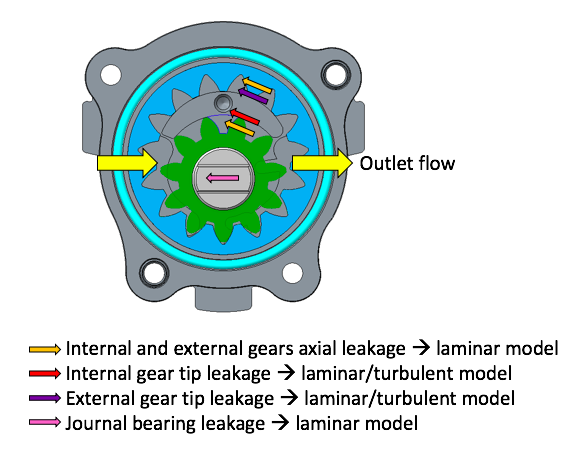
\includegraphics[width=0.9 \linewidth]{flow.png}
    \label{fig:em}
\end{figure}
La freccia rosa al centro ("\textit{journal bearing leakage}") indica uno scentramento del più piccolo ingranaggio centrale rispetto alla posizione originaria. Le frecce rossa e viola disegnano rispettivamente lo sfalsamento interno ed esterno della componente superiore definita "a mezza luna" (nell'ambito delle cosiddette distanze di punta). Infine, le due frecce arancioni rappresentano una variazione delle distanze assiali interna ed esterna.\\
La produzione GP5 può essere dunque distinta in "classi di coefficiente di perdita", ossia gruppi di pompe che condividono lo stesso \textit{leakage coefficient} $\alpha$, che viene messo in relazione con la pressione e la portata con la seguente formula\footnote{$Q_{GP}$ e $P_{out}$ sono note rispettivamente col nome di \texttt{media\_portata\_velocita\_1}, e \texttt{media\_pressione\_velocita\_1}} verificata sperimentalmente:
\begin{equation}
    Q_{GP} = Q_{GP,theor} − \alpha \cdot P_{out}
\end{equation}
L'andamento del coefficiente di perdita, poiché fondamentale per il monitoraggio del prodotto, verrà analizzato non soltanto al variare del programma selezionato o della fase impostata, ma soprattutto in relazione alle altre misurazioni estratte durante il circuito pneumatico di prova. Nel dettaglio, a ciascuna delle due fasi di test sono associate interessanti osservazioni numeriche relative a picco e media della \textit{outlet pression}, picco e media della portata in uscita, picco e media della coppia in fase finale - ovvero in corrispondenza di una velocità di 100 rotazioni al minuto -, e temperatura di prova del liquido con cui viene lubrificata la pompa per la rotazione.
\\
Altre variabili significative sono presenti nel \textit{database} fornito, tra cui il codice dei turni in cui è suddivisa la linea di lavoro, ora e data del \textit{record}, descrizione dell'esito finale della prova, e il \textit{Programma}, corrispondente alla classe di prodotto GP5, che è raggruppabile nelle due macro-categorie \textit{Daimler (DAI} e Standard (STD)\footnote{La macro-categoria \textit{Daimler} è descritta dal codice programma \texttt{18\_GP5\_910\_CW}, mentre la tipologia Standard comprende tutti gli altri codici programma}.\\
\\
A partire da tale caso di studio, sono stati proposti tre \textit{task}:
\begin{enumerate}
    \item analisi preliminare delle grandezze del processo produttivo e implementazione di un sistema di monitoraggio \textit{real-time} del coefficiente di perdita (Sezioni \ref{prem} e \ref{rt})
    \item definizione, dato un intervallo del coefficiente di perdita, di un limite dinamico della portata $Q_{GP}$ rispetto alla pressione in uscita (Sezione \ref{lim})
    \item stima di un modello efficace per la previsione del coefficiente di perdita $\alpha$ (Sezione \ref{Mod}).
\end{enumerate}
%------------------------------------------------
\section{Data Preparation}
Il \textit{database} si compone di 296605 osservazioni, descritte da 33 colonne. Tuttavia, è stato necessario focalizzare l'analisi su quelle che presentavano un certo grado di rilevanza e utilità per l'oggetto di studio. Ciò ha comportato la rimozione, durante una prima fase di \textit{pre-processing}, delle variabili che presentavano le seguenti caratteristiche: si manifestavano come un unico valore costante\footnote{Le costanti rimosse sono: \texttt{"Banco"}, \texttt{"Master"}, \texttt{"Picco coppia zero"}, \texttt{"Picco coppia iniziale"}, \texttt{"Media coppia iniziale"}, \texttt{"Velocità 1"}, \texttt{"Picco pressione velocità 2"}, \texttt{"Media pressione velocita 2"}, \texttt{"Picco portata velocità 2"}, \texttt{"Media portata velocità 2"}.}, mostravano una distribuzione eccessivamente sbilanciata verso una sola classe\footnote{È questo il caso di \texttt{"Velocità 2"}, \texttt{"Esito"} e di conseguenza \texttt{"N. Esito"}, \texttt{"Coppia max ciclo"}, \texttt{"Velocità a regime"}.}, erano ridondanti, poco interessanti o erano già state segnalate tali dai fornitori del \textit{dataset}\footnote{Le colonne inutili sono: \texttt{"Codice da Linea"} - identificativo del pezzo -, \texttt{"Media coppia zero"}, \texttt{'Data'} e \texttt{'Ora'}, poiché i dati sono stati raccolti in un arco temporale non uniforme.}.\\
Successivamente, è stata rimossa una riga, poiché penalizzata dalla mancanza dei valori di pressione. Infine, poiché la differenza di scala era spesso eccessiva per molte colonne numeriche, si è deciso di normalizzare la matrice originale, mappando tutte le variabili non categoriche fra 0 e 1. 
%------------------------------------------------
\section{Analisi preliminari}\label{prem}
Dopo le operazioni di pulizia appena menzionate, si è proceduto ad analizzare in maniera preliminare le colonne rilevanti, per ottenere un primo approfondimento sui descrittori e i rapporti di dipendenza fra gli stessi. 
\subsection{Variabili categoriche}
I dati nominali conservati sono relativi a due precisi aspetti del processo: la segmentazione del lavoro in turni differenti e il programma selezionato per la creazione del pezzo, ovvero la tiplogia di pompa.\\
Per quanto riguarda la prima, è stato necessario aggregare le medesime classi registrate erroneamente in maniera diversa, uniformandone la denominazione. In questo modo, sono state ottenute 5 classi: "A", "B", "C", "D", "0". Le ultime due, poiché osservate in minor misura e non specificate inizialmente dai fornitori del \textit{dataset}, sono state etichettate come \textit{missing values}.
\begin{figure}[h]
    \centering
    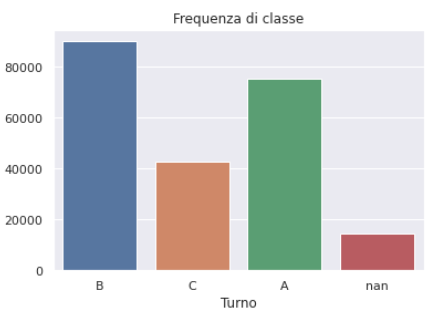
\includegraphics[width=0.9 \linewidth]{turno.png}
    \label{fig:em}
    \caption{\textit{Bar chart} per la visualizzazione delle rispettive frequenze osservate dei turni.}
\end{figure}
Come osservabile in Figura 1, i principali blocchi in cui è organizzato il processo presentano una frequenza diversa: il turno "B" costituisce più del 40\% dei \textit{records}, "A" si presenta nel $\sim$34\% dei casi e "C" nel $\sim$19\%.\\
La composizione del "Programma" mostra un fortissimo sbilanciamento verso la classe GP5 denominata \texttt{18\_GP5\_910\_CW} (Figura 2), che corrisponde alla pompa "\textit{Daimler}". Le restanti tipologie, raggruppate sotto denominazione "Standard", formano in totale meno del 23\% dei casi e sono principalmente rappresentate dalle categorie \texttt{17\_GP5\_430\_CCW} (10.6\%) e \texttt{12\_GP5\_430B\_D1} (8.5\%).
\begin{figure}[h]
    \centering
    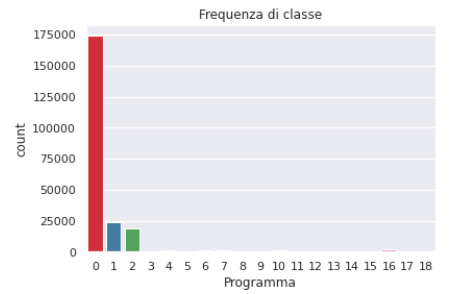
\includegraphics[width=0.9 \linewidth]{prog.png}
    \label{fig:em}
    \caption{\textit{Bar chart} per la visualizzazione delle rispettive frequenze osservate dei programmi.}
\end{figure}
Per una visualizzazione migliore, in Figura 3 è riassunta la distribuzione delle frequenze logaritmiche delle varie classi GP5.
\begin{figure}[h]
    \centering
    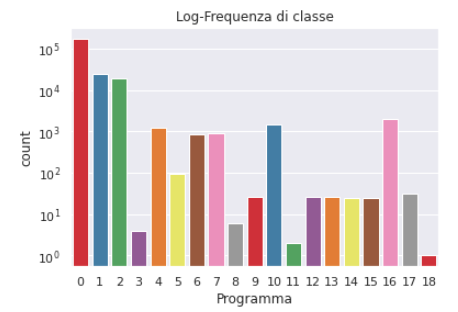
\includegraphics[width=0.9 \linewidth]{proglog.png}
    \label{fig:em}
    \caption{\textit{Bar chart} per la visualizzazione delle rispettive frequenze logaritmiche dei programmi.}
\end{figure}
\\
Tra le variabili categoriche esaminate, "Esito" descrive le eventuali - rarissime - imperfezioni del prodotto. A tal proposito, il 99.5\% delle volte il risultato è ottimale, mentre l'anomalia più comune è indicata come "scarto picco coppia max fase pulizia iniziale" (0.1\% delle osservazioni).
\subsection{Variabili numeriche}
I dati numerici registrano, per ogni pompa, due principali set di valori, relativi al picco e alla media di pressione (in bar) e portata (in litri all'ora), misurati in corrispondenza di due velocità diverse:
\begin{itemize}
    \item a regime: 2300 \textit{r.p.m}
    \item 140 \textit{r.p.m}
\end{itemize}
Si vedrà che, a prescindere dalla velocità, le due grandezze condividono un'elevatissima dipendenza lineare.
\subsubsection{Descrittori della pressione}
Innanzitutto, le grandezze relative al picco e alla media hanno una distribuzione multimodale nell'ambito di entrambe le misurazioni della velocità (Figura 4), rivelando picchi di diversa altezza. Il range osservato è molto superiore per quanto concerne la velocità a regime (come riassunto dalla Tabella 1). Inoltre, le distribuzioni dei valori appaiono quasi identiche per classe di velocità, rivelando una fortissima similarità fra l'andamento del picco e e della pressione media (Figura 5).
\begin{figure}[h]
    \centering
    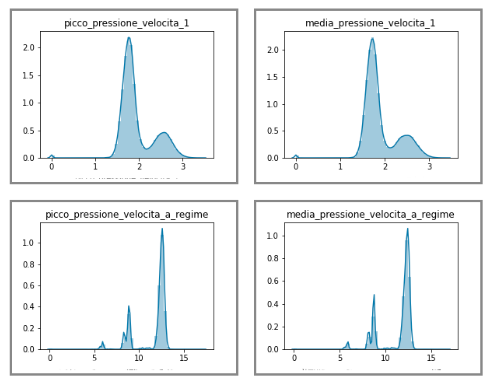
\includegraphics[width=1 \linewidth]{press.png}
    \label{fig:em}
    \caption{Distribuzioni delle grandezze relative alla pressione.}
\end{figure}
\begin{figure}[h]
    \centering
    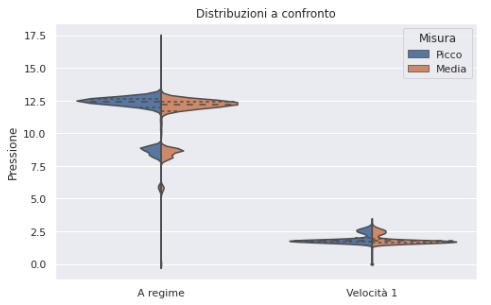
\includegraphics[width=1 \linewidth]{p.png}
    \label{fig:em}
    \caption{Distribuzioni delle grandezze relative alla pressione, in corrispondenza della velocità "1" e a regime, appaiate nell'ambito della stessa misurazione. È possibile notare sia la superiorità della pressione a regime, che la fortissima vicinanza dell'andamento del picco rispetto alla pressione media.}
\end{figure}
{\begin{table}[h]
\centering
\begin{tabular}[t]{lccc}
\toprule
Pressione&Minimo&Media&Massimo\\
\midrule
\textbf{Picco (140)}&0.19&1.94&3.45\\
\textbf{Picco (2300)}&5.38&11.61&14.21\\
\textbf{Media (140)}&0.1&1.88&3.38\\
\textbf{Media (2300)}&5.33&11.41&14.01\\
\bottomrule
\end{tabular}
\caption{Rassunto relativo alla media e al range dei valori di pressione.}
\end{table}}
\subsubsection{Descrittori della portata}
Le rispettive distribuzioni di portata (Figura 6) rivelano andamenti molto meno regolari. In particolare, i \textit{records} a regime sono caratterizzati da una coda molto estesa verso destra, lasciando presupporre la presenza di una  quota rilevante di valori anomali e permettendo di intravedere una differenza ancor più ampia rispetto a quanto visto con una velocità di 140 \textit{r.p.m}.  
\begin{figure}[h]
    \centering
    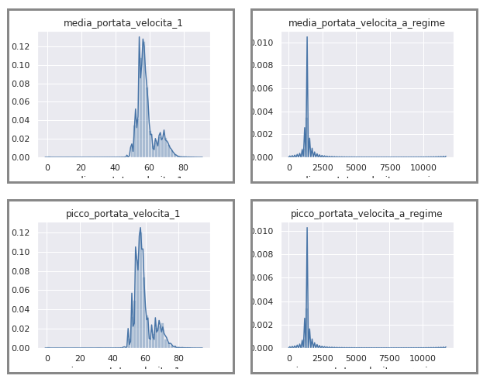
\includegraphics[width=1 \linewidth]{port.png}
    \label{fig:em}
    \caption{Distribuzioni delle grandezze relative alla portata.}
\end{figure}
{\begin{table}[h]
\centering
\begin{tabular}[t]{lccc}
\toprule
Portata&Minimo&Media&Massimo\\
\midrule
\textbf{Picco (140)}&30.30&58.96&93.6\\
\textbf{Picco (2300)}&930.5&1309.6&1422.9\\
\textbf{Media (140)}&28.07&58.5&90\\
\textbf{Media (2300)}&927.63&1304.8&1416.2\\
\bottomrule
\end{tabular}
\caption{Rassunto relativo alla media e al range dei valori di portata.}
\end{table}}
I comportamenti mostrati dalle osservazioni relative alla pressione della pompa si ritrovano in forma identica esaminando le misurazioni di portata: anche qui, esiste una grandissima somiglianza fra le distribuzioni di picco e media, e - come anticipato - una differenza di scala ancor più ampia fra i valori estratti per le due velocità (Figura 7).
\begin{figure}[h]
    \centering
    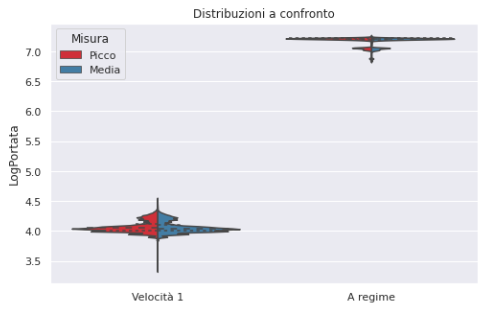
\includegraphics[width=1 \linewidth]{port2.png}
    \label{fig:em}
    \caption{Distribuzioni delle grandezze relative alla portata, in corrispondenza della velocità "1" e a regime, appaiate nell'ambito della stessa misurazione. Poichè la differenza era troppo grande per permettere una visualizzazione comprensibile, è stato necessario adottare una scala logaritmica.}
\end{figure}
\\
Infine, è interessante notare come le colonne relative alla pressione e alla portata condividano dipendenze lineari con grado molto elevato, come visibile in Figura 8: la correlazione assoluta media raggiunge addirittura un livello di $\sim$0.95, con un minimo di 0.79 - tra i picchi di portata misurati fra le due velocità - e 8 collinearità perfette. In particolare, oltre alla quasi identicità delle distribuzioni nell'ambito della stessa grandezza - menzionata in precedenza -, appaiono interessanti le seguenti dipendenze lineari:
\begin{itemize}
    \item picco pressione e picco portata, entrambi alla velocità di 140 \textit{r.p.m.} ($\sim$0.91)
    \item media pressione e picco portata, sempre per quanto riguarda la fase di controllo ($\sim$0.91)
    \item media portata e picco pressione, a 140 \textit{r.p.m.} ($\sim$0.92)
    \item media portata e media pressione, per la fase di controllo ($\sim$0.92)
    \item media pressione e media portata a velocità di regime, fra cui s'individua una correlazione perfetta
    \item picco pressione e picco portata a velocità di regime, sempre una correlazione perfetta
    \item picco portata e media pressione a velocità di regime: perfetta collinearità.
\end{itemize}
\begin{figure}[h]
    \centering
    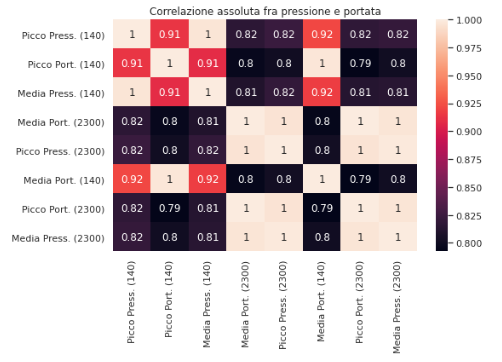
\includegraphics[width=1 \linewidth]{corrpp.png}
    \label{fig:em}
    \caption{Matrice di correlazione, con valori assoluti, fra tutte le variabili di pressione e portata.}
\end{figure}
Appare quindi evidente la sistematica dipendenza fra pressione e portata, che, osservando i dati forniti, paiono spesso essere state generate dalla stessa distribuzione casuale, a prescindere dalla misura scelta e dalla fase impostata. Per questa ragione, in fase di generazione dei modelli di regressione, la matrice del disegno potrebbe essere affetta da un eccessivo problema di multicollinearità, rischiando di divenire quasi-singolare o addirittura non invertibile, penalizzando una stima corretta sia dei coefficienti di regressione che degli indici di bontà di adattamento della funzione di regressione. Sarà pertanto necessario rimuovere tali variabili più correlate, oppure adottare strategie utili alla selezione di un modello a più bassa dimensionalità, come, ad esempio, le tipologie \textit{Ridge} e \textit{Lasso}.
\subsubsection{Altre variabili}
Le altre colonne numeriche, filtrate dalla fase di \textit{pre-processing} e ritenute rilevanti ai fini dello studio, sono: media coppia in fase finale (100 \textit{rpm}), picco coppia in fase finale e temperatura di prova del liquido.\\
Per quanto riguarda la prima, la distribuzione è fortemente asimmetrica verso valori elevati, con una discreta porzione di \textit{outliers}. Il picco della stessa grandezza presenta una coda ancor più lunga (in scala logaritmica in Figura 9). Medesima condizione di elevata asimmetria vale per la temperatura, compresa fra un range di $37.61^°$ e $49.1^°$.
\begin{figure}[h]
    \centering
    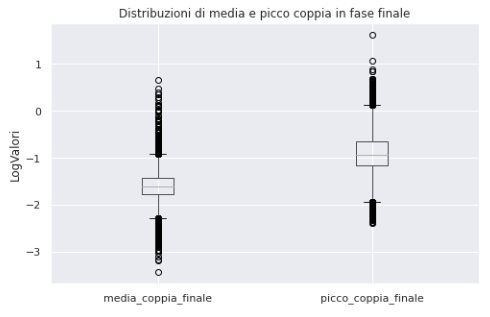
\includegraphics[width=1 \linewidth]{cf.png}
    \label{fig:em}
    \caption{\textit{Boxplot} per la visualizzazione della distribuzione delle variabili "Media coppia finale" e "Picco coppia finale".}
\end{figure}
È importante citare che anche fra la media e il picco della coppia in fase finale (100 \textit{rpm}) esista una forte dipendenza lineare positiva ($\sim$0.83). Bisognerà pertanto valutare questa ulteriore collinearità in fase di stima del modello per la previsione del coefficiente.\\
Al contrario, queste due variabili non presentano un'elevata dipendenza rispetto i dati di pressione e portata: la correlazione rimane sempre ben al di sotto del 20\%. Lo stesso vale per i valori di temperatura.

\subsection{Target: coefficiente di dispersione}\label{Alpha}
Il coefficiente di dispersione è calcolato con la formula
\begin{equation}\label{eq}
    \alpha=\frac{108.36-\text{Media portata (@140)}}{\text{Media pressione (@140)}}
\end{equation}
e i valori sono compresi in un range molto ampio, fra un minimo di $\sim$5.7 e un massimo di $\sim$817, con media e mediana rispettivamente pari a $\sim$27.8 e $\sim$29.43. La distribuzione è sbilanciata verso alti valori, come visibile in Figura 10.
\begin{figure}[h]
    \centering
    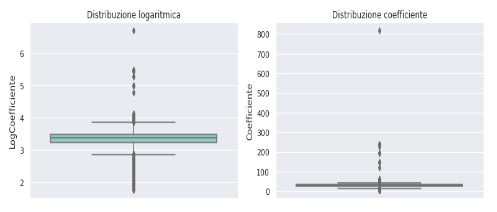
\includegraphics[height=100,width=1 \linewidth]{coeff.png}
    \label{fig:em}
    \caption{Distribuzione del coefficiente di \textit{leakage} in scala logaritmica e originale.}
\end{figure}
In Figura, è possibile notare una certa concentrazione dei \textit{records} in un intervallo di ampiezza ridotta attorno alla mediana. Questa considerazione è appurata dal basso coefficiente di variazione: $\sim$0.26.\\
Poiché il coefficiente di \textit{leakage} è indice della performance della pompa prodotta, è ragionevole supporre che ad ogni classe GP5, come conseguenza della differenza fra le proprie caratteristiche di progettazione e quelle delle altre categorie, si associ un diverso livello di prestazione - quindi un diverso \textit{range} di $\alpha$. Da un'analisi grafica superficiale (Figura 11), questa assunzione appare corretta: le distribuzioni del coefficiente, raggruppate per "Programma", appaiono spesso distanti, facendo ipotizzare l'esistenza di una notevole variabilità fra i gruppi, potenzialmente interessante per la costruzione di un modello predittivo. 
\begin{figure}[h]
    \centering
    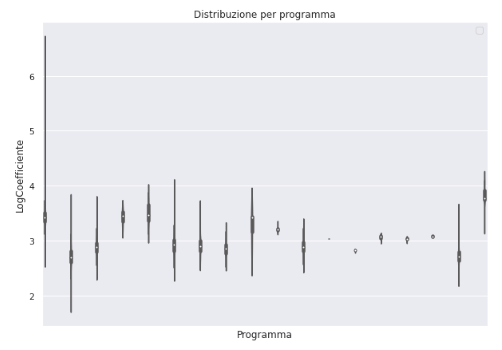
\includegraphics[width=1 \linewidth]{Programma.png}
    \label{fig:em}
    \caption{Distribuzioni del coefficiente $\alpha$ raggruppate per classe GP5 ("Programma").}
\end{figure}
Inoltre, è possibile che tale varianza fra le classi GP5 si manifesti non solo fra i livelli di performance, ma anche fra i coefficienti di regressione delle variabili esplicative scelte. In altre parole, è probabile che la selezione di un determinato Programma comporti una relazione significativamente diversa - rispetto agli altri tipi di pompe - fra $\alpha$ e le altre grandezze. Se questa ipotesi venisse verificata, allora si potrebbe dimostrare quanto il contributo delle varie parti coinvolte nel processo - monitorate attraverso la misurazione dei valori registrati nelle colonne nel database - si modifichi, influenzato dagli specifici fattori contestuali relativi alla diversa progettazione di ogni classe di pompa. In questo modo, sarebbe anche possibile ottimizzare il valore del coefficiente $\alpha$, monitorando questi fattori in maniera differente a seconda del Programma. Pertanto, con lo scopo di analizzare in maniera più approfondita la variabilità della funzione di regressione lineare di $\alpha$ in base al tipo di pompa in produzione, si è scelto di stimare una tipologia di modello misto adatta ai dati influenzati da effetti contestuali: il cosiddetto \textit{multilevel model}. Tale approfondimento è trattato nella Sezione \ref{Mod}.\\
Oltre alla relazione con "Programma", il coefficiente di dispersione mostra un collinearità molto elevata con molte altre colonne. Tralasciando le distribuzioni da cui $\alpha$ è stato generato (equazione \ref{eq}), le variabili con cui è più fortemente correlato sono relative alla pressione a regime ("Picco pressione velocita a regime" al 75\% e "Media pressione velocita a regime" al 74.6\%) e al picco di portata durante la stessa fase (74\%). Normalmente, queste dovrebbero essere quindi incluse nel \textit{subset} dei candidati esplicativi per la regressione lineare di $\alpha$, poiché potrebbero contribuire ad una stima accurata. Tuttavia, come si vedrà nella Sezione \ref{Mod}, la \textit{feature selection} sarà un'operazione difficile, a causa della multicollinearità rilevata fra le misurazioni di portata e pressione - in entrambe le fasi - e del conseguente rischio di ottenere una matrice del disegno quasi-singolare o invertibile. Ad esempio, se si volessero includere entrambe le variabili di pressione in fase di regime, la penalizzazione alla correttezza del modello non deriverebbe soltanto dalla loro reciproca collinearità, bensì anche dalla loro dipendenza lineare con le colonne utilizzate per calcolare $\alpha$.\\
La correlazione mostrata da $\alpha$ rispetto a "Media coppia finale" appare moderata (16.9\%), e "Picco coppia finale" ha una dipendenza lineare pari a circa il 7\%. È necessario ricordare che anche fra queste due grandezze esiste una collinearità rischiosa, la quale, nel caso in cui esse venissero incluse assieme nel modello, finirebbe per distorcere i coefficienti di regressione. Infine, la correlazione rispetto alla temperatura è ridotta: -6.9\%.\\
In seguito, poiché le osservazioni erano corredate da dati temporali relativi alla data - giorno, mese e anno - e all'orario, si è proceduto a verificare la possibilità di estrarre eventuali trend temporali. Tuttavia, le misurazioni appaiono cronologicamente disomogenee su due livelli. Innanzitutto, i \textit{record} nono sono stati forniti con coerenza temporale per quanto riguarda l'anno (Figura 12). 
\begin{figure}[h]
    \centering
    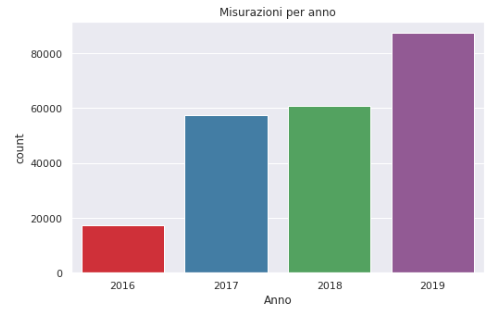
\includegraphics[width=1 \linewidth]{anno.png}
    \label{fig:em}
    \caption{Frequenza delle misurazioni per anno. I dati non sono stati forniti in maniera omogenea.}
\end{figure}
In ogni caso, non è comunque visibile alcuna differenza significativa fra le distribuzioni della performance nei vari anni (Figura 13).
\begin{figure}[h]
    \centering
    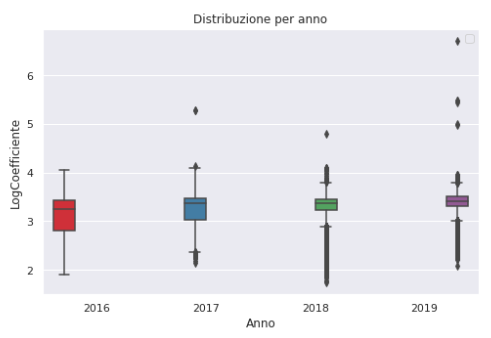
\includegraphics[width=1 \linewidth]{anno1.png}
    \label{fig:em}
    \caption{Distribuzioni del coefficiente $\alpha$ raggruppate per anno.}
\end{figure}
\\
Neppure per quanto riguarda il mese, le registrazioni sono omogenee, come visibile in Figura 14.
\begin{figure}[h]
    \centering
    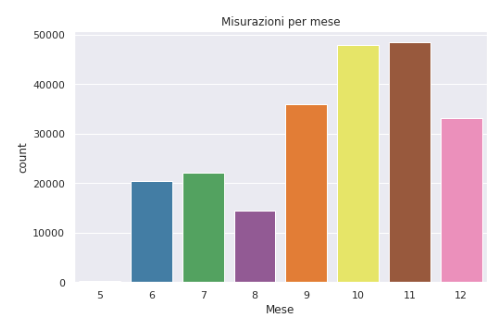
\includegraphics[width=1 \linewidth]{mese.png}
    \label{fig:em}
    \caption{Frequenza delle misurazioni per mese. I dati non solo non sono stati forniti in maniera omogenea, ma i primi 4 mesi sono addirittura mancanti, e maggio non riporta quasi osservazioni.}
\end{figure}
\\
Eppure, nonostante dalla collezione dei dati possa sembrare impossibile estrarre una certa periodicità per i motivi appena spiegati, l'andamento del coefficiente di dispersione è inaspettatamente armonico (Figura 15).
\begin{figure}[h]
    \centering
    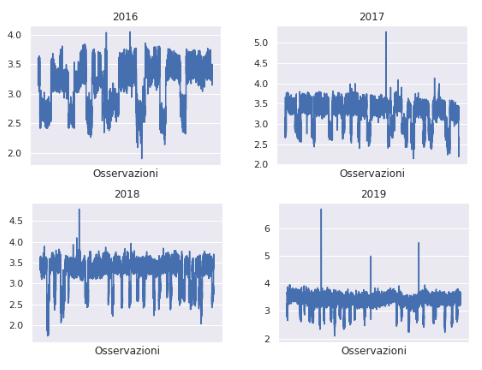
\includegraphics[width=1 \linewidth]{anni.png}
    \label{fig:em}
    \caption{Andamento del coefficiente di dispersione $\alpha$ per anno.}
\end{figure}
Tuttavia, è sufficiente eseguire un clustering grafico dei punti in base al programma di appartenenza per dedurre la motivazione di tale apparente periodicità: essa non deriva da un'autocorrelazione temporale fra i valori del coefficiente, bensì dall'ordine con cui è stato scelto di effettuare le misurazioni sui diversi gruppi GP5, che, come si è visto in precedenza, hanno distribuzioni differenti. L'andamento, perciò, appare generato da una sinusoide solamente perché le osservazioni alternano classi di pompa con performance elevate a categorie con un $\alpha$ minore. Quanto detto è evidente in Figura 16.
\begin{figure}[h]
    \centering
    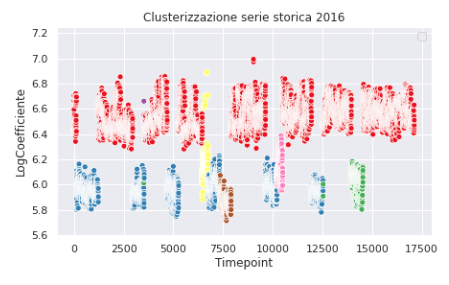
\includegraphics[width=1 \linewidth]{Cluster.png}
    \label{fig:em}
    \caption{Andamento del coefficiente di dispersione $\alpha$ durante l'anno 2016, clusterizzato in base alla variabile "Programma". Il colore rosso indica la tiplogia di pompa \textit{Daimler} - la più popolosa -, mentre gli altri colori sono associati alle sottocategorie Standard.}
\end{figure}

\subsection{\textit{Outliers Detection}}
L'ultima fase di analisi preliminare consiste nell'identificazione degli \textit{outliers}. Grazie ad essa, è possibile, in una fase di ottimizzazione della produzione, ricostruire il trend del processo, individuare le anomalie non segnalate dalla variabile "Esito" ed inferire eventuali fattori in grado di causarle. Innanzitutto, si è proceduto ad estrarre gli \textit{outliers} univariati all'interno della distribuzione del coefficiente di dispersione $\alpha$. Per farlo, poichè è stato verificato che tale distribuzione non fosse di tipo Normale, è stato applicato il metodo non parametrico della distanza interquartile, segnalando pertanto i punti inferiori a k volte il primo quartile e superiori a k volte il terzo quartile, con $k = 1.5$. È stato appurato che queste anomalie non dipendono da un particolare programma\footnote{Le anomalie sono presenti sia in corrispondenza della categoria \textit{Daimler} sia Standard.}, né si verificano in particolari anni o mesi.
\begin{figure}[h]
    \centering
    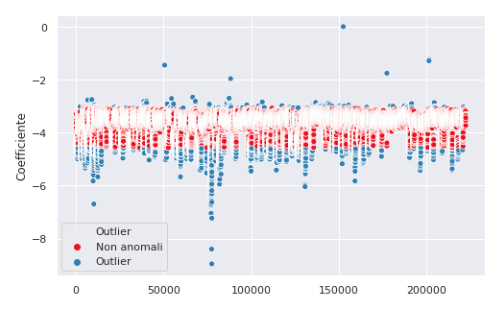
\includegraphics[width=1 \linewidth]{out.png}
    \label{fig:em}
    \caption{Identificazione degli outlier univariati all'interno della distribuzione del coefficiente di dispersione.}
\end{figure}
\\
Si è successivamente proceduto ad estrarre \textit{outlier} multivariati grazie all'algoritmo \textit{Local Outlier Factor} (LOF), basato sul calcolo delle deviazioni locali di ogni punto dal proprio vicinato. In questo caso, i valori anomali individuati rappresentano un porzione molto grande del database (75\%) e prescindono, come in precedenza, da particolari condizioni o programmi. Questa elevata quantità può dipendere dall'incidenza che gli specifici fattori contestuali di progettazione hanno sulle varie distribuzioni, elevando il grado di variabilità nell'andamento globale, così come dall'alternanza di fasi diverse nel processo. Sarebbe pertanto più utile applicare l'algoritmo di \textit{anomaly detection} separatamente in corrispondenza della cosiddetta velocità 1 (140rpm) e della fase di regime, e su ciascuna classe GP5.
%------------------------------------------------
\section{Sistema di monitoraggio \textit{real-time}}\label{rt}
Il processo industriale può essere ottimizzato grazie all'implementazione di sistemi di monitoraggio che individuino in tempo reale le eventuali anomalie, registrino i dati e li rappresentino graficamente su schermo per ottenere una visualizzazione \textit{user-friendly} dell'andamento delle variabili rilevanti. Nell'ambito di questo progetto, viene proposta una soluzione in grado di eseguire automaticamente le attività elencate. Tale sistema è stato interamente scritto e testato all'interno dell'ambiente di programmazione \texttt{Python}\footnote{Il codice è disponibile al seguente link: \url{https://github.com/RCrvro/Industry-Lab---Progetto/tree/master/Monitoraggio\%20realtime}.}.\\
Il programma, dunque, consta di tre elementi principali. Innanzitutto, si ha una componente di \textit{data ingestion}, la quale permette di ricevere il flusso di dati osservati dai sensori durante il processo di creazione di ogni pompa, ed elaborarlo per due scopi separati:
    \begin{itemize}
        \item rendere i dati adatti alla proiezione grafica sullo schermo;
        \item registrare metadati relativi alle misurazioni ricevute, \textit{timestamp} e valore decodificato, e segnalare se tale dato consiste in un \textit{outlier} univariato, aggiornando ad ogni \textit{step} il calcolo del metodo della distanza interquartile. 
    \end{itemize}
Questa operazione è stata simulata attraverso il client del \textit{software} \texttt{Apache Kafka}\footnote{Documentazione ufficiale del client di \texttt{Apache Kafka} in \texttt{Python}: \url{https://pypi.org/project/kafka-python/}.}, che si presta perfettamente al \textit{task} definito: si configura, infatti, come una piattaforma \textit{open source} a bassissima latenza per la gestione di \textit{feed} in tempo reale. Grazie al suo utilizzo, il sistema è in grado di ricevere grandi moli di osservazioni in intervalli di tempo molto ridotti, effettuare le elaborazioni prima citate ad altissima velocità e visualizzare il risultato grafico senza dover ritardare o ricaricare l'applicazione, e senza che l'utente debba controllare le operazioni in \textit{background}. Nel dettaglio, il sensore invia le misurazioni attraverso un \texttt{Producer} di \texttt{Apache Kafka}, e il sistema, connettendosi a un \texttt{Consumer}, effettua una lettura continua di questi dati all'interno del \textit{topic} in cui sono stati memorizzati. La lettura di un nuovo valore comporta, poi, l'estrazione dei metadati. Ad ogni sensore verrà applicato un \texttt{Producer} diverso, e per ciascuno verrà aperta una connessione verso il sistema tramite un \texttt{Consumer} separato, in modo da mantenere le letture indipendenti ed evitare un sovraccarico.\\
Il secondo elemento consiste in una componente grafica, curata mediante i \textit{tool} di visualizzazione forniti dall'interfaccia \texttt{Dash} di \texttt{Plotly}\footnote{Documentazione ufficiale di \texttt{Dash}: \url{https://plotly.com/dash/}.}. Essa riceve i valori letti dalla \textit{topic} di \texttt{Apache Kafka} e aggiorna in tempo reale due tipologie di visualizzazione per i dati inviati dai sensori: un \textit{BoxPlot} per monitorare la distribuzione totale, e un grafico \textit{LineChart} per l'andamento.\\
Infine, la terza componente - nominata "\texttt{writer}"\footnote{Il codice del "\texttt{writer}" è disponibile al link: \url{https://github.com/RCrvro/Industry-Lab---Progetto/blob/master/Monitoraggio\%20realtime/writer.py}.} - esegue un programma indipendente, che registra i metadati - \textit{timestamp}, dato numerico e segnalazione di eventuali valori anomali - all'interno di un database locale. Quest'ultimo, dunque, svolgerà la funzione di \textit{logfile} del processo. 
\subsection{Demo}
È disponibile una demo del sistema di monitoraggio al link \href{https://youtu.be/R7GCE91WyMc}{\textbf{\texttt{youtu.be/R7G}}}. 
\\
In questo caso, si è scelto di simulare la visualizzazione di ipotetiche osservazioni relative al coefficiente di dispersione $\alpha$ (in verde) e alla media di portata a 140rpm (in arancione), perché, essendo variabile soggetta a limiti imposti in fase di produzione, appare ragionevole monitorarla in tempo reale.\\
Nel video, sul lato destro dello schermo, sono visibili quattro pagine del terminale. La prima in alto esegue un \texttt{Producer} per simulare l'invio delle misurazioni del coefficiente $\alpha$ da parte del proprio sensore, tramite scrittura manuale di alcuni valori. La seconda attiva un secondo \texttt{Producer}, per simulare il sensore della variabile di portata. La terza implementa il programma \texttt{writer}: ogni dato ricevuto dal sensore - in questo caso di $\alpha$ - viene scritto, assieme ai metadati, nel \textit{logfile} \texttt{"Coefficiente.csv"} apparso sul bordo destro del monitor dopo l'invio del primo valore. Alla fine del video, il file verrà aperto, per mostrare il risultato delle registrazioni. Inoltre, sempre per quanto concerne il \texttt{writer}, la pagina mostrerà un conteggio dei messaggi ricevuti. Infine, l'ultima finestra in basso inizializza l'applicazione grafica in corrispondenza della porta \texttt{8050} e mantiene connesso il sistema di monitoraggio.\\
L'applicazione è programmata per la segnalazione di eventuali errori, che possono essere esaminati cliccando l'icona blu nell'angolo inferiore destro della pagina \textit{Web}. 
%------------------------------------------------
\section{Limite dinamico di portata}\label{lim}
Poiché la \textit{performance} della pompa GP5 dipende strettamente dal proprio valore di portata in uscita, è necessario controllare che tale misurazione non scenda al di sotto di una determinata soglia, variabile a seconda della macro-categoria selezionata: \textit{Daimler} o Standard\footnote{I valori corretti di portata in uscita per la pompa \textit{Daimler} sono compresi fra 45.86 e 63.36. Per quanto riguarda la categoria Standard, gli estremi considerati sono 57.36 e 75.36.}. Oltre al tipo di "programma", però, tale grandezza condivide una relazione matematica con le variabili del coefficiente di \textit{leakage} $\alpha$ e della pressione (equazione \ref{eq}). Pertanto, il processo produttivo necessita di un monitoraggio dei valori di portata in uscita rispetto alle colonne menzionate. A tal proposito, oltre ad un algoritmo che calcoli, a partire da $\alpha$ e pressione, la portata in uscita e valuti se tale misurazione rientra nel \textit{range} definito dalla miglior\footnote{La regione ammissibile viene limitata superiormente perché eventuali valori oltre il migliore registrato potrebbero derivare da anomalie del pezzo prodotto.} e peggior osservazione in corrispondenza della categoria GP5, è possibile rappresentare graficamente tale limite dinamico come una regione ammissibile all'interno di uno spazio tridimensionale, e osservare la differenza fra il piano e una data misurazione. In questo modo, è possibile monitorare già graficamente la presenza di eventuali anomalie, e si è in grado di valutare visivamente la distanza dai comportamenti tipici del processo produttivo.\\
È disponibile una demo dell'algoritmo di rappresentazione grafica del limite dinamico di portata al link \href{https://www.youtube.com/watch?v=cxHw8cPm-Ek}{\textbf{\texttt{youtu.be/cxH}}}: date in input le coordinate di $\alpha$ e pressione, viene generata la regione ammissibile prima descritta (in blu) e indicato il punto relativo all'osservazione. La regione critica si modifica a seconda della categoria di pompa, e il colore del punto varia in base alla correttezza dell'osservazione fornita in input: se essa rientra nel limite indicato per la data classe GP5, il punto è rappresentato in verde (Figura 18), altrimenti in rosso (Figura 19).
\begin{figure}[h]
    \centering
    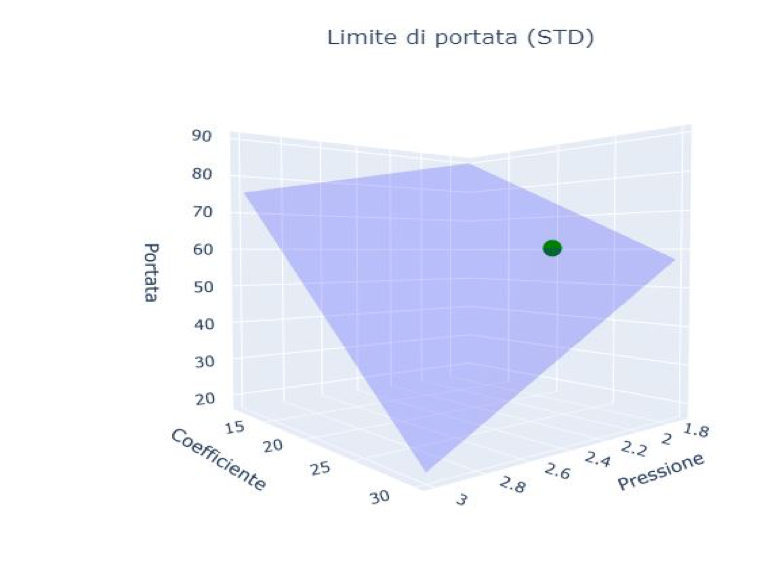
\includegraphics[width=0.9 \linewidth]{STD.png}
    \label{fig:em}
    \caption{Il punto osservato è compreso nella regione ammissibile. Ciò significa che i valori di coefficiente di dispersione, pressione e soprattutto portata - in funzione di essi - sono da considerarsi regolari. Il punto è pertanto colorato in verde.}
\end{figure}
\begin{figure}[h]
    \centering
    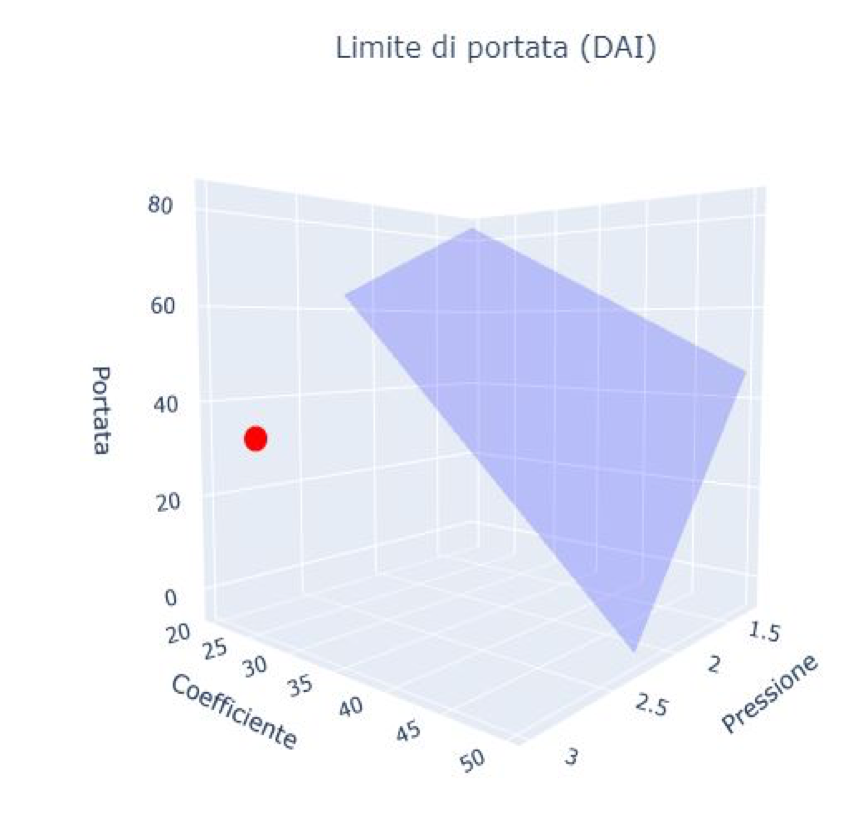
\includegraphics[width=0.9 \linewidth]{DAI.png}
    \label{fig:em}
    \caption{Il punto osservato non è compreso nella regione ammissibile. Ciò significa che l'osservazione è anomala, ed è pertanto segnalata in rosso.}
\end{figure}
%----------------------------------------------------------------------------------------
\section{Modelli di previsione}\label{Mod}
La previsione del coefficiente di perdita $\alpha$ (\textit{leakage coefficient}) è stata effettuata utilizzando tre diverse tecniche di regressione: 
\begin{enumerate}
    \item Modello OLS per regressione lineare multipla
    \item Tecniche di \textit{shrinkage}: regressione \textit{Ridge} e \textit{Lasso}
    \item Modello misto: regressione \textit{multilevel}
\end{enumerate}
\subsection{Modelli OLS}
La regressione lineare rappresenta un metodo di stima del valore atteso condizionato di una variabile - dipendente (o endogena) -, dati i valori di altre variabili indipendenti (o esogene), assumendo pertanto l'esistenza di una relazione lineare tra le $X$ e
la variabile target $Y$. La formulazione è rappresentata dalla seguente equazione:
\begin{equation}\label{eq}
    Y = \beta_{0} + \beta_{1}x_{1} + \beta_{n}x_{n} + u_{i}
\end{equation}
dove:
\begin{itemize}
    \item $\beta_{0}$ è l'intercetta della retta di regressione, ovvero il valore atteso di $Y$ quando le altre variabili indipendenti sono pari a zero
    \item $\beta_{1}$, $\beta_{n}$ sono i coefficienti angolari della retta di regressione, interpretabili come pesi di rilevanza assegnati a ciascuna \textit{feature}
    \item $u_{i}$ è l'errore statistico.
\end{itemize}
Come discusso in precedenza, le variabili di portata e pressione si distribuiscono quasi identicamente, sia per quanto riguarda le diverse fasi - di controllo e a regime -, sia per quanto concerne le due diverse misurazioni di media e picco. Pertanto, si è proceduto inizialmente a stimare alcun modelli per la previsione del coefficiente di \textit{leakage} $\alpha$ mantenendo separate le variabili di portata e di pressione. Inoltre, dato che la collinearità tra tali colonne avrebbe potuto causare una sottostima della significatività delle $X$ e una sovrastima dell'indice di bontà di adattamento $R^2$, si è deciso di includere soltanto le grandezze di pressione e portata che presentavano una correlazione pari o inferiore all'82\%.\\
La significatività statistica delle variabili verrà estratta dal confronto fra il \textit{p-value}, ($Pr(>|t|)$), e il livello di significatività statistica, prefissato 0.05. Il risultato della regressione è quindi basato sull’ipotesi che i coefficienti di regressione associati alle variabili siano nulli, contrapposta all'ipotesi alternativa, per cui essi non sono uguali a zero ed esiste cioè una relazione tra la $Y$ e il regressore selezionato. Più precisamente, soltanto quando $\text{\textit{p-value}} < 0.05$ i $\beta$ sono significativamente diversi da zero, pertanto rilevanti. Nelle tabelle con cui verranno esposti i risultati di ogni modello OLS, il grado di significatività - che dipende dall'ordine della differenza fra il \textit{p-value} e il limite prefissato - sarà indicato da alcuni asterischi: maggiore il numero degli stessi, da un minimo di zero a un massimo di 3, maggiore la rilevanza della variabile in questione per la previsione della $Y$.\\
Per migliorare la stima della funzione di regressione e dell'indice $R^2$ per ciascun modello \textit{ordinary least squares}, è stata applicata la tecnica \textit{k-folds cross validation} (con $k=5$): i dati sono suddivisi iterativamente in \textit{training} e \textit{test set}, ristimando e valutando k volte il modello ottenuto, in modo da evitare problemi di sovradattamento e campionamento asimmetrico.\\
Le prossime sezioni riassumono i risultati ottenuti da ciascun modello.
\subsubsection{Modello OLS con variabili di portata}
\textbf{Modello 1}: Coefficiente $\sim$  Picco Port. (140) + Media Port.(2300) + Picco Port. (2300) + Temperatura + Media Coppia Finale
{\begin{table}[h] 
\centering
\begin{tabular}[t]{lccc}
\toprule 
Variabile&$Pr(> |t|)$&Coefficiente\\
\midrule 
\textbf{Intercetta}&$<$2e-16 ***&0.04440\\ 
\textbf{Picco Port. (140)}&$<$2e-16 ***&-0.07284\\ 
\textbf{Media Port. (2300)}&$<$2e-16 ***&-0.18002\\ 
\textbf{Picco Port. (2300)}&$<$2e-16 ***&0.20332\\ 
\textbf{Temperatura}&$<$2e-16 ***&-0.00152\\
\textbf{Media Coppia Finale}&$<$2e-16 ***&0.01893\\
\bottomrule 
\end{tabular}
\end{table}}\\
Per la previsione del coefficiente di \textit{leakage} sono state utilizzate, oltre alle variabili di portata che presentano una reciproca correlazione inferiore al 82\%, le variabili "Temperatura" e "Media Coppia Finale"\footnote{\label{cf1}Nel modello non vengono mai incluse entrambe le variabili relative alla coppia finale, perchè presentano una correlazione eccessiva e rischiano pertanto di compromettere la correttezza delle stime.}. Tutte le variabili risultano statisticamente significative con grado molto elevato. La variabile più rilevante per la previsione di $\alpha$ si rivela essere \textit{Picco Port. (2300)}, con un coefficiente di regressione pari a $\sim$0.2. Inoltre, è possibile notare una relazione negativa tra la variabile target e le seguenti covariate: picco di portata in fase di controllo (140 rpm), media di portata in fase a regime (2300 rpm) e temperatura. Il coefficiente di determinazione ($R^2$) associato al modello è abbastanza buono, pari a 0.8737.\\
\\
\textbf{Modello 2}: Coefficiente $\sim$  Picco Port. (140) + Media Port.(2300) + Picco Port. (2300) + Temperatura + Picco Coppia Finale
{\begin{table}[h] 
\centering
\begin{tabular}[t]{lccc}
\toprule 
Variabile&$Pr(> |t|)$&Coefficiente\\
\midrule 
\textbf{Intercetta}&$<$2e-16 ***&0.045667\\ 
\textbf{Picco Port. (140)}&$<$2e-16 ***&-0.073420\\ 
\textbf{Media Port. (2300)}&$<$2e-16 ***&-0.202027\\ 
\textbf{Picco Port. (2300)}&$<$2e-16 ***&0.225690\\ 
\textbf{Temperatura}&$<$2e-16 ***&-0.001174\\
\textbf{Picco Coppia Finale}&$<$2e-16 ***&0.007755\\
\bottomrule 
\end{tabular}
\end{table}}\\
A differenza del precedente caso, la generazione di un modello di previsione del coefficiente ha implicato la sostituzione di "Picco Coppia Finale" a "Media Coppia Finale". Anche qui, tutte le variabili risultano statisticamente significative con grado identicamente elevato. La variabile più rilevante è ancora il picco di portata in fase a regime, caratterizzato da un leggero aumento del proprio coefficiente di regressione. Il coefficiente di determinazione ($R^2$) associato al modello è leggermente inferiore al precedente: 0.872.\\
\\
In seguito, si è proceduto a combinare le colonne relative alla coppia finale - considerate separatamente\footnote{Nota precedente.} - e alla temperatura con le singole grandezze di portata che mostravano una correlazione $\leq 82\%$.\\
\\
\textbf{Modello 3}: Coefficiente $\sim$  Picco Port. (140) + Temperatura + Media Coppia Finale
{\begin{table}[h] 
\centering
\begin{tabular}[t]{lccc}
\toprule 
Variabile&$Pr(> |t|)$&Coefficiente\\
\midrule 
\textbf{Intercetta}&$<$2e-16 ***&0.076790\\ 
\textbf{Picco Port. (140)}&$<$2e-16 ***&-0.106135\\
\textbf{Temperatura}&$<$2e-16 ***&-0.005642\\
\textbf{Media Coppia Finale}&$<$2e-16 ***&0.033331\\
\bottomrule 
\end{tabular}
\end{table}}\\
Tutte le variabili mostrano un grado di significatività statistica molto elevato. La variabile più rilevante è il picco di portata in fase di controllo, che presenta una relazione negativa con il \textit{coefficiente}. La motivazione, qui, è ovvia: il picco di portata in fase di controllo è identicamente distribuito alla media di portata a 140 rpm e correlato al 91\% con la media di pressione in fase di controllo, che sono le due variabili con cui $\alpha$ è stato generato (equazione \ref{eq}). Il coefficiente di determinazione ($R^2$) si abbassa ancora: $\sim$0.81.\\
\\
\textbf{Modello 4}: Coefficiente $\sim$  Picco Port. (140) + Temperatura + Picco Coppia Finale
{\begin{table}[h] 
\centering
\begin{tabular}[t]{lccc}
\toprule 
Variabile&$Pr(> |t|)$&Coefficiente\\
\midrule 
\textbf{Intercetta}&$<$2e-16 ***&0.07968\\ 
\textbf{Picco Port. (140)}&$<$2e-16 ***&-0.10728\\
\textbf{Temperatura}&$<$2e-16 ***&-0.00495\\
\textbf{Picco Coppia Finale}&$<$2e-16 ***&0.01119\\
\bottomrule 
\end{tabular}
\end{table}}\\
Tutte le variabili risultano statisticamente molto significative. La variabile più rilevante è ancora, per le ragione ovvie prima menzionate, il picco di portata in fase di controllo. Il coefficiente di determinazione ($R^2$) è pari a 0.803.\\ 
\\
\textbf{Modello 5}: Coefficiente $\sim$ Media Port.(2300) + Temperatura + Media Coppia Finale 
{\begin{table}[h] 
\centering
\begin{tabular}[t]{lccc}
\toprule 
Variabile&$Pr(> |t|)$&Coefficiente\\
\midrule 
\textbf{Intercetta}&$<$2e-16 ***&-0.0103293\\ 
\textbf{Media Port. (2300)}&$<$2e-16 ***&0.0479580\\
\textbf{Temperatura}&$<$0.0128 *&-0.0003287\\
\textbf{Media Coppia Finale}&$<$2e-16 ***&0.0368901\\
\bottomrule 
\end{tabular}
\end{table}}\\
In questo caso, la variabile "Temperatura" rivela livello di significatività nettamente minore rispetto alle altre variabili. Nonostante le altre variabili risultano rilevanti per determinare il valore di $\alpha$, la capacità del modello nel catturare la variabilità dei dati subisce comunque una grave diminuzione, producendo un $R^2$ pari a 0.7443.\\
\\
\textbf{Modello 6}: Coefficiente $\sim$ Media Port.(2300) + Temperatura + Picco Coppia Finale
{\begin{table}[h] 
\centering
\begin{tabular}[t]{lccc}
\toprule 
Variabile&$Pr(> |t|)$&Coefficiente\\
\midrule 
\textbf{Intercetta}&$<$2e-16 ***&-0.00876\\ 
\textbf{Media Port. (2300)}&$<$2e-16 ***&0.04856\\
\textbf{Temperatura}&0.333\\
\textbf{Picco Coppia Finale}&$<$2e-16 ***&0.02097\\
\bottomrule 
\end{tabular}
\end{table}}\\
La variabile "Temperatura" non risulta essere statisticamente significativa: il \textit{p-value} ad essa associato è molto superiore al limite di 0.05, per cui l'ipotesi nulla che il suo coefficiente di regressione sia nullo non viene rifiutata. Si è dunque proceduto a ristimare la funzione di regressione senza tale colonna, ottenendo un $R^2$ di 0.7393.\\
\\
\textbf{Modello 7}: Coefficiente $\sim$ Picco Port. (2300) + Temperatura + Media Coppia Finale
{\begin{table}[h] 
\centering
\begin{tabular}[t]{lccc}
\toprule 
Variabile&$Pr(> |t|)$&Coefficiente\\
\midrule 
\textbf{Intercetta}&$<$2e-16 ***&-0.0105056\\ 
\textbf{Picco Port. (2300)}&$<$2e-16 ***&0.0486005\\
\textbf{Temperatura}&0.342\\
\textbf{Media Coppia Finale}&$<$2e-16 ***&0.0342434\\
\bottomrule 
\end{tabular}
\end{table}}\\
Anche qui, la temperatura non risulta rilevante ai fini della previsione e viene nuovamente scartata. Le altre \textit{feature} contribuiscono in misura ridotta alla determinazione del coefficiente.
L'indice di bontà di adattamento ($R^2$) associato al modello è pari a 0.7450919.\\
\\
\textbf{Modello 8}: Coefficiente $\sim$ Picco Port. (2300) + Temperatura + Picco Coppia Finale
{\begin{table}[h] 
\centering
\begin{tabular}[t]{lccc}
\toprule 
Variabile&$Pr(> |t|)$&Coefficiente\\
\midrule 
\textbf{Intercetta}&$<$2e-16 ***&-0.00904\\ 
\textbf{Picco Port. (2300)}&$<$2e-16 ***&0.04919\\
\textbf{Temperatura}&0.728\\
\textbf{Picco Coppia Finale}&$<$2e-16 ***&0.01982\\
\bottomrule 
\end{tabular}
\end{table}}\\
La "Temperatura" non risulta nuovamente significativa. Come in precedenza, le altre variabili sono poco rilevanti e producono un $R^2$ di $\sim$0.74.
\subsubsection{Modelli di previsione con variabili di pressione}
\textbf{Modello 1}: Coefficiente $\sim$  Picco Press. (140) + Media Press.(2300) + Picco Press. (2300) + Temperatura + Media Coppia Finale
{\begin{table}[H] 
\centering
\begin{tabular}[t]{lccc}
\toprule 
Variabile&$Pr(> |t|)$&Coefficiente\\
\midrule 
\textbf{Intercetta}&$<$2e-16 ***&0.065700\\ 
\textbf{Picco Press. (140)}&$<$2e-16 ***&-0.080396\\ 
\textbf{Media Press. (2300)}&$<$2e-16 ***&-0.025513\\ 
\textbf{Picco Press. (2300)}&$<$2e-16 ***&0.036890\\ 
\textbf{Temperatura}&0.241\\
\textbf{Media Coppia Finale}&$<$2e-16 ***&-0.001809\\
\bottomrule 
\end{tabular}
\end{table}}
La variabile "Temperatura" non risulta statisticamente significativa e viene dunque scartata per la previsione del coefficiente di perdita. Al contrario, i valori dei coefficienti di regressione associati alle altre variabili risultano molto rilevanti nella previsione del \textit{leakage coefficient}. Il modello offre un'ottima misura di performance ($R^2$), pari a 0.9507.\\
\\
\textbf{Modello 2}: Coefficiente $\sim$  Picco Press. (140) + Media Press.(2300) + Picco Press. (2300) + Temperatura + Picco Coppia Finale
{\begin{table}[h] 
\centering
\begin{tabular}[t]{lccc}
\toprule 
Variabile&$Pr(> |t|)$&Coefficiente\\
\midrule 
\textbf{Intercetta}&$<$2e-16 ***&0.065649\\ 
\textbf{Picco Press. (140)}&$<$2e-16 ***&-0.080372\\ 
\textbf{Media Press. (2300)}&$<$2e-16 ***&-0.024678\\ 
\textbf{Picco Press. (2300)}&$<$2e-16 ***&0.036036\\ 
\textbf{Temperatura}&0.0614\\
\textbf{Picco Coppia Finale}&$<$2e-16 ***&-0.001603\\
\bottomrule 
\end{tabular}
\end{table}}\\
La temperatura continua ad essere eliminata in quanto non significativa e viene eliminata dal modello. Le altre variabili, invece, contribuiscono efficacemente alla descrizione dell'andamento di $\alpha$: il coefficiente di determinazione ($R^2$) è pari a 0.9508.\\
Tuttavia, è possibile che il fattore penalizzante della multicollinearità, da cui è affetta la matrice del disegno, distorca i rispettivi risultati della regressione. Per tale ragione, è stato necessario valutare successivi modelli, che includono separatamente le grandezze di pressione con una correlazione $\leq 82\%$, combinate con "Temperatura", "Media Coppia Finale" e "Picco Coppia Finale". Le due variabili relative alla coppia finale continuano ad essere considerate separatamente per i motivi prima espresse.\\
\\
\textbf{Modello 3}:  Coefficiente $\sim$  Picco Press. (140) + Temperatura + Media Coppia Finale
{\begin{table}[h] 
\centering
\begin{tabular}[t]{lccc}
\toprule 
Variabile&$Pr(> |t|)$&Coefficiente\\
\midrule 
\textbf{Intercetta}&$<$2e-16 ***&0.0829343\\ 
\textbf{Picco Press. (140)}&$<$2e-16 ***&-0.0968194\\
\textbf{Temperatura}&$<$2e-16 ***&-0.0007664\\
\textbf{Media Coppia Finale}&$<$2e-16 ***&-0.0021630\\
\bottomrule 
\end{tabular}
\end{table}}\\
Tutte le variabili sono statisticamente significative. La variabile più rilevante per prevedere il coefficiente di perdita è il picco di pressione in fase di controllo (140 rpm), caratterizzato da una relazione negativa con $\alpha$. La ragione, come visto in precedenza, è facilmente deducibile: tale colonna è identicamente ditribuita alla media di pressione durante la medesima fase e correlata al 92\% con la media di portata a 140 rpm, le due variabili con cui la $Y$ è stata generata (equazione \ref{eq}). l coefficiente di determinazione ($R^2$) associato al modello è pari a 0.938.\\
\\
\textbf{Modello 4}: Coefficiente $\sim$  Picco Press. (140) + Temperatura + Picco Coppia Finale
{\begin{table}[h] 
\centering
\begin{tabular}[t]{lccc}
\toprule 
Variabile&$Pr(> |t|)$&Coefficiente\\
\midrule 
\textbf{Intercetta}&$<$2e-16 ***&0.082962\\ 
\textbf{Picco Press. (140)}&$<$2e-16 ***&-0.096812\\
\textbf{Temperatura}&$<$2e-16 ***&-0.000584\\
\textbf{Picco Coppia Finale}&$<$2e-16 ***&-0.003744\\
\bottomrule 
\end{tabular}
\end{table}}\\
Tutte le variabili sono statisticamente significative e caratterizzate da una relazione negativa con il coefficiente di dispersione. Come ci si poteva attendere, "Picco Press. (140)" risulta ancora la più rilevante. La bontà di adattamento rimane eccellente: 0.938.\\
\\
\textbf{Modello 5}:  Coefficiente $\sim$ Media Press.(2300) + Temperatura + Media Coppia Finale
{\begin{table}[h] 
\centering
\begin{tabular}[t]{lccc}
\toprule 
Variabile&$Pr(> |t|)$&Coefficiente\\
\midrule 
\textbf{Intercetta}&$<$2e-16 ***&-0.007341\\ 
\textbf{Media Press. (2300)}&$<$2e-16 ***&0.048612\\
\textbf{Temperatura}&0.00271 **&-0.000396\\
\textbf{Media Coppia Finale}&$<$2e-16 ***&0.036867\\
\bottomrule 
\end{tabular}
\end{table}}\\
Qui, la variabile "Temperatura" è leggermente meno significativa, e con molta probabilità questo fattore è causa della riduzione della capacità del modello di catturare la variabilità dei dati, offrendo un $R^2$ di $\sim$0.745.\\
\\
\textbf{Modello 6}: Coefficiente $\sim$ Media Press.(2300) + Temperatura + Picco Coppia Finale
{\begin{table}[h] 
\centering
\begin{tabular}[t]{lccc}
\toprule 
Variabile&$Pr(> |t|)$&Coefficiente\\
\midrule 
\textbf{Intercetta}&$<$2e-16 ***&-0.00876\\ 
\textbf{Media Press. (2300)}&$<$2e-16 ***&0.04856\\
\textbf{Temperatura}&0.333\\
\textbf{Picco Coppia Finale}&$<$2e-16 ***&0.02097\\
\bottomrule 
\end{tabular}
\end{table}}\\
In questo caso, la temperatura non è addirittura significativa per la previsione del target, e viene dunque scartata dal modello. A seguito di quanto detto, è facile dedurre la ragione per cui il coefficiente di correlazione ($R^2$) subisca un'ulteriore contrazione a $\sim$0.74.\\
\\
\textbf{Modello 7}: Coefficiente $\sim$ Picco Press.(2300) + Temperatura + Media Coppia Finale
{\begin{table}[h] 
\centering
\begin{tabular}[t]{lccc}
\toprule 
Variabile&$Pr(> |t|)$&Coefficiente\\
\midrule 
\textbf{Intercetta}&$<$2e-16 ***&-0.0071346\\ 
\textbf{Picco Press. (2300)}&$<$2e-16 ***&0.0488265\\
\textbf{Temperatura}&0.000201 ***&-0.0004871\\
\textbf{Media Coppia Finale}&$<$2e-16 ***&0.0316346\\
\bottomrule 
\end{tabular}
\end{table}}\\
Tutte le variabili sono statisticamente significative. Nonostante ciò, l'indice di bontò di adattamento ($R^2$) è basso: 0.7487.\\
\\
\textbf{Modello 8}: Coefficiente $\sim$ Picco Press.(2300) + Temperatura + Picco Coppia Finale
{\begin{table}[h] 
\centering
\begin{tabular}[t]{lccc}
\toprule 
Variabile&$Pr(> |t|)$&Coefficiente\\
\midrule 
\textbf{Intercetta}&$<$2e-16 ***&-0.0058528\\ 
\textbf{Picco Press. (2300)}&$<$2e-16 ***&0.0493986\\
\textbf{Temperatura}&0.00187**&-0.0004141\\
\textbf{Picco Coppia Finale}&$<$2e-16 ***&0.0194586\\
\bottomrule 
\end{tabular}
\end{table}}\\
Tutte le variabili sono rilevanti, ma, come visto nel modello 7, la performance ($R^2$) è più scarsa (0.745).
\subsection{Tecniche di \textit{shrinkage}}
Poichè i dati presentano un fortissimo problema di multicollinearità, risulta impossibile includere la totalità delle colonne in un modello di regressione lineare per la previsione del coefficiente $\alpha$, ed è quindi necessario ridurre la matrice del disegno. L'estrazione di un subset ottimale di \textit{feature} può avvenire tramite vari tentativi di selezione manuale - come effettuato nella sezione precedente -, ma tale metodo può essere troppo dispendioso. In alternativa, è possibile eseguire una \textit{feature selection} implicita tramite aggiunta di una componente di penalizzazione alla funzione di regressione. L'applicazione di questo meccanismo di regolarizzazione, ponendo un vincolo al valore dei coefficienti di regressione, contrae le stime $\beta$ e quindi riduce la rilevanza dei candidati esplicativi. In questo modo, le colonne che meno contribuiscono a descrivere la variabilità di $\alpha$, subiscono un'ulteriore riduzione della propria importanza. Qualora la contrazione comportasse l'annullamento di un coefficiente di regressione, allora il predittore associato sarebbe indirettamente scartato dal modello. In questo caso, le tecniche di \textit{shrinkage} avranno successo se riusciranno a filtrare le poche colonne realmente importanti, eliminando l'informazione ridondante presente nelle distribuzioni eccessivamente correlate.\\
Sono state adottate due popolari tipologie di regolarizzazione: \textit{Ridge} e \textit{Lasso}.
\subsubsection{Regressione \textit{Ridge}}
La stimatore lineare \textit{Ridge} \cite{Ridge} è formulato come segue:
\begin{equation}\label{eq}
    \hat{\beta}^{\lambda}=(X'X+\lambda I_p)^{-1}X'y
\end{equation}
dove $\lambda$ è il parametro di regolarizzazione pari alla norma $L_2$, tale per cui:
\begin{itemize}
    \item se $\lambda=0$, la soluzione coincide con il quella derivante dal metodo ai minimi quadrati ordinari;
    \item se $\lambda>0$, si produce una penalizzazione sul punto di minimo della funzione di perdita $D_{Ridge}^{(\beta,\lambda)}$.
\end{itemize}
In questo modo, la complessità del modello diminuisce senza eliminare nessuna variabile.\\
Il valore atteso $\mathbb{E}[\hat{\beta}^{\lambda}]$ si dimostra essere pari a
\begin{equation}
   (X'X+\lambda I_p)^{-1}(X'X)\beta\neq\beta 
\end{equation}
, dimostrando quindi che $\hat{\beta}^{\lambda}$ è distorto. Tuttavia, nonostante l'introduzione del \textit{bias} appena menzionato, è possibile dimostrare come questa tecnica di \textit{shrinkage}, oltre ad avere l'effetto di risolvere efficacemente la supercollinearità fra i regressori, riesca a produrre, per un'opportuna scelta di $\lambda$, un errore quadratico medio dello stimatore minore rispetto a quello offerto dal metodo OLS.\\
Dunque, per uno stimatore ridge, la selezione di un buon valore per $\lambda$ è fondamentale: per trovare l'ottimo è stata utilizzato un metodo di ricerca a griglia (\textit{Grid Search}), ottenendo un parametro quasi nullo, pari cioè a 0.01. Poichè la penalizzazione applicata è quasi nulla, è possibile dedurre che, nonostante le aspettative, la regolarizzazione offerta da una norma $L_2$ sia quasi inutile. Precisamente, nel modello sono state considerate congiuntamente tutte le variabili originarie - relative a pressione e portata, temperatura, e coppia finale. I risultati ottenuti sono riassunti in Figura 20.
\begin{figure}[h]
    \centering
    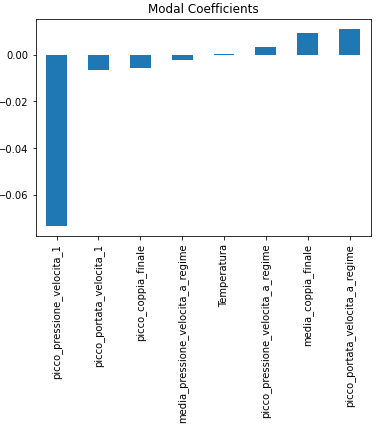
\includegraphics[width=0.7 \linewidth]{ridge.png}
    \label{fig:em}
    \caption{Stime \textit{Ridge} dei coefficienti di regressione.}
\end{figure}
È possibile notare come la variabile "Picco Press. (140)" risulti la più rilevante, ovvero la meno contratta dalla penalizzazione. La ragione risiede, come spiegato in precedenza, nella fortissima dipendenza lineare fra tale regressore e le distribuzioni con cui è stato generato il coefficiente di dispersione. Al contrario, la "Temperatura" non contribuisce alla previsione, e il suo $\beta$ è pertanto annullato. Per il resto, la relativa importanza del resto dei candidati appare nettamente ridimensionata, ad indicare la grande ridondanza informativa all'interno della matrice del disgeno. Infine, il coefficiente di determinazione ($R^2$) associato al modello è pari a 0.845, attestandosi pertanto su un livello accettabile, ma non eccellente.
\subsubsection{Regressione \textit{Lasso}}
Nonostante sia un'ottima soluzione per contrarre la varianza della funzione di regressione, il metodo \textit{Ridge} è, in realtà, raramente in grado di effettuare una vera e propria \textit{feature selection}, ovvero di annullare i coefficienti che moltiplicano le variabili meno rilevanti per descrivere il fenomeno di studio. Questa limitazione deriva dalla scelta di una norma $L_2$ come componente di penalizzazione. La regressione \textit{Lasso} \cite{Lasso} può essere pertanto utilizzata come alternativa ai metodi di \textit{feature selection}, perché, utilizzando una funzione di regolarizzazione non derivabile - norma $L_1$, è in grado di ridurre ulteriormente i coefficienti di regressione verso lo zero. Anche qui, la selezione del valore ottimale di $\lambda$ è stata effettuata utilizzando un metodo di ricerca a griglia (\textit{Grid Search}), ottenendo un parametro ottimo praticamente nullo (0.00001). Le stime \textit{Lasso} dei coefficienti sono rappresentate graficamente in Figura 21.
\begin{figure}[h]
    \centering
    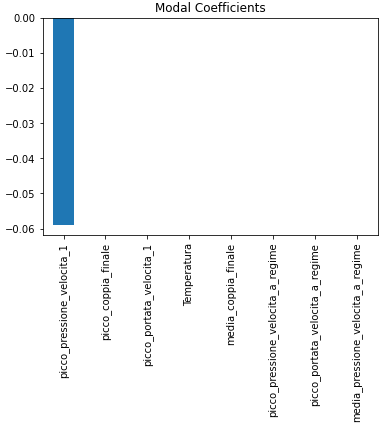
\includegraphics[width=0.7 \linewidth]{lasso.png}
    \label{fig:em}
    \caption{Stime \textit{Lasso} dei coefficienti di regressione.}
\end{figure}
L'unica variabile ritenuta importante per la previsione di $\alpha$ è sempre il picco di pressione in fase di controllo (140 rpm). Ogni altro candidato è scartato, come conseguenza logica dell'eccessiva dipendenza fra tutte le principali misurazioni che descrivono il processo di produzione delle pompe GP5. L'indice di bontà di adattamento ($R^2$) è scarso, pari a 0.7058.
\subsection{Regressione Multilevel}
I \textit{Multilevel Model} \cite{Multil}\cite{Multil1}, noti anche come gerarchici lineari, sono modelli statistici caratterizzati da parametri che variano su più livelli. Come anticipato nella Sezione \ref{Alpha}, i dati a disposizione - riguardanti principalmente le performance del prodotto - variano a seconda dei sottogruppi di pompe. La regressione \textit{Multilevel} appare quindi perfetta per il fenomeno di studio, permettendo di considerare nel modello finale i fattori contestuali che subentrano nei diversi programmi di produzione, ovvero le differenti relazioni, da gruppo a gruppo, fra la variabile target e i regressori $X$.\\
Sono stati pertanto costruiti vari modelli multilivello, considerando separatamente le variabili di pressione e portata - sempre con lo scopo di gestire il problema di multicollinearità - , oltre agli altri candidati esplicativi gà menzionati. La variabile di \textit{grouping} "Programma"\footnote{Con "variabile di \textit{grouping}" s'intende la colonna con cui vengono raggruppate le osservazioni, con lo scopo di ottenere una stima gerarchica, ovvero estrarre i diversi vettori dei coefficienti di regressione per ciascun gruppo.}, è indicata nella formulazione del modello con la scrittura "$(1|\textit{Programma})"$\footnote{Il valore 1 prima del simbolo $\mid$ sta ad indicare la stima di un'intercetta.}. 
\subsubsection{Modelli multilivello con variabili di portata}
\textbf{Modello 1}:  Coefficiente $\sim$  Picco Port. (140) + Media Port.(2300) + Picco Port. (2300) + Temperatura + Media Coppia Finale + (1$\mid$Programma)
{\begin{table}[h] 
\centering
\begin{tabular}[t]{lccc}
\toprule 
Variabile&$Pr(> |t|)$\\
\midrule 
\textbf{Intercetta}&$<$2e-16 ***&\\
\textbf{Picco Port. (140)}&$<$2.2e-16 ***\\ 
\textbf{Media Port. (2300)}&$<$2.2e-16 ***\\ 
\textbf{Picco Port. (2300)}&$<$2.2e-16 ***\\ 
\textbf{Temperatura}&$<$2.2e-16 ***\\
\textbf{Media Coppia Finale}&$<$2.2e-16 ***\\
\bottomrule 
\end{tabular}
\end{table}}\\
Tutte le variabili risultano statisticamente significative. Il coefficiente di determinazione ($R^2$) associato al modello è elevato, pari a 0.918.
È possibile misurare la differenza dei gruppi di programma, in termine di diversa funzione di regressione che mette in relazione le variabili indipendenti con $\alpha$, considerando il valore del coefficiente di dispersione, la $Y$, come somma di tre componenti:
\begin{equation}
    y_{ij}=\mu+a_j+\varepsilon_{ij}
\end{equation}
dove
\begin{itemize}
    \item $y_{ij}$ è l'i-esima osservazione nel j-esimo gruppo 
    \item $\mu$ è interpretabile come valore atteso globale di tutti i dati originari
    \item $a_j$ è l'effetto casuale che caratterizza tutte le osservazioni di un dato gruppo, interpretabile pertanto come l'influenza che i fattori contestuali hanno sulle misurazioni della classe j, ovvero lo scostamento del gruppo j-esimo rispetto a trend globale
    \item $\varepsilon_{ij}$ è il rumore casuale proprio della data osservazione.
\end{itemize}
Nella stima di un classico modello di regressione lineare, il fattore contestuale $a_j$ è assunto nullo, poichè non viene ipotizzata l'esistenza di una gerarchia. Nel caso di una regressione multilivello, invece, il grado in cui i fattori contestuali comportano dinamiche diverse all'interno dei gruppi è misurato dal rapporto fra la varianza degli effetti casuali $\sigma_a$ e la varianza totale dei dati (come somma di $\sigma_a$ e la varianza del rumore casuale di ogni osservazione $\sigma_{\varepsilon}$:
\begin{equation}
    \frac{\sigma_a}{\sigma_a+\sigma_{\varepsilon}}
\end{equation}
Pertanto, al crescere di questo indice, cresce la certezza nell'affermare l'esistenza di una gerarchia sistematica all'interno dei dati.\\
In questo caso, il valore del coefficiente di correlazione intraclasse (ICC), pari a 0.912, conferma l'ipotesi formulata, ovvero che il coefficiente di dispersione $\alpha$ possa essere descritto similmente nell'ambito di ciascun programma e in maniera significativamente diversa tra le varie classi. La presenza di gruppi significativamente diversi rispetto al trend globale, ovvero di classi GP5 che subiscono scostamenti rilevanti a causa dei propri fattori contestuali di produzione, può essere verificata graficamente come in Figura 22.
\begin{figure}[H]
    \centering
    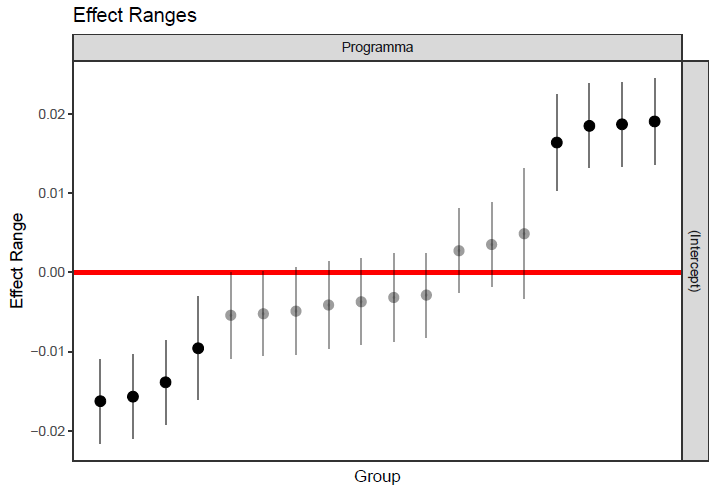
\includegraphics[width=0.7 \linewidth]{multi1.png}
    \label{fig:em}
    \caption{Grafico per la visualizzazione della significatività dell'effetto casuale di gruppo $a_j$.}
\end{figure}
I punti in tale rappresentazione indicano il valore dell'effetto casuale di ciascun gruppo $a$; se l'intervallo di confidenza attorno all'effetto casuale $a_j$ comprende lo zero - ovvero interseca la linea rossa in Figura -, allora significa che la classe j-esima non subisce uno scostamento significativo rispetto al trend globale, cioè che i propri fattori contestuali non causano la formazione di un cluster di produzione a sé stante. Al contrario, se l'intervallo di confidenza si allontana dallo zero, allora il gruppo può considerarsi parte di una gerarchia sistematica sottostante ai dati. Qui, il numero di cluster di produzione è pari a 8 su 18.
\textbf{Modello 2}: Coefficiente $\sim$  Picco Port. (140) + Media Port.(2300) + Picco Port. (2300) + Temperatura + Picco Coppia Finale + (1$\mid$Programma)
{\begin{table}[h] 
\centering
\begin{tabular}[t]{lccc}
\toprule 
Variabile&$Pr(> |t|)$\\
\midrule 
\textbf{Intercetta}&$<$2e-16 ***&\\
\textbf{Picco Port. (140)}&$<$2.2e-16 ***\\ 
\textbf{Media Port. (2300)}&$<$2.2e-16 ***\\ 
\textbf{Picco Port. (2300)}&$<$2.2e-16 ***\\ 
\textbf{Temperatura}&$<$2.2e-16 ***\\
\textbf{Picco Coppia Finale}&$<$2.2e-16 ***\\
\bottomrule 
\end{tabular}
\end{table}}\\
Tutte le variabili risultano statisticamente significative. Il coefficiente di determinazione ($R^2$) associato al modello è pari a 0.921. L'esistenza di una gerarchia nei dati è riconfermata, anche in questo caso, dall'elevato coefficiente di correlazione intraclasse (ICC): 0.915, e dalla presenza di effetti contestuali significativi in 9 cluster, visibili in Figura 23.
\begin{figure}[H]
    \centering
    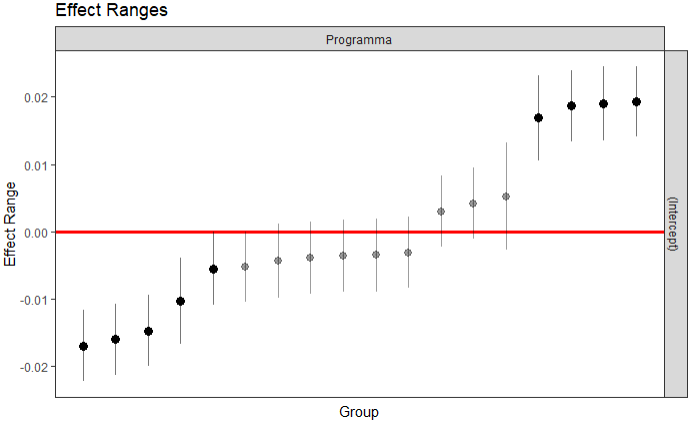
\includegraphics[width=0.7 \linewidth]{multi2.png}
    \label{fig:em}
    \caption{Grafico per la visualizzazione della significatività dell'effetto casuale di gruppo $a_j$.}
\end{figure}
\subsubsection{Modelli di previsione con variabili di pressione}
\textbf{Modello 1}: Coefficiente $\sim$  Picco Press. (140) + Media Press.(2300) + Picco Press. (2300) + Temperatura + Media Coppia Finale + (1$\mid$Programma)
{\begin{table}[h] 
\centering
\begin{tabular}[t]{lccc}
\toprule 
Variabile&$Pr(> |t|)$\\
\midrule 
\textbf{Intercetta}&$<$2e-16 ***&\\
\textbf{Picco Press. (140)}&$<$2.2e-16 ***\\ 
\textbf{Media Press. (2300)}&$<$2.2e-16 ***\\ 
\textbf{Picco Press. (2300)}&$<$2.2e-16 ***\\ 
\textbf{Temperatura}&0.9759\\
\textbf{Media Coppia Finale}&0.1177\\
\bottomrule 
\end{tabular}
\end{table}}\\
Le variabili \textit{Temperatura} e \textit{Media Coppia Finale} non risultano statisticamente significative e sono dunque scartate. Nonostante il minor numero di predittori, il coefficiente di determinazione ($R^2$) associato al modello è superiore a quanto visto nell'ambito delle misurazioni di portata, pari a 0.939. Il valore del coefficiente di correlazione intraclasse (ICC) è, tuttavia, nettamente inferiore: 0.797. Ciò indica che le relazioni fra le grandezze di pressione - in combinazione con gli altri candidati - e la variabile target $\alpha$ variano in maniera decisamente minore fra le varie classi di pompa rispetto a quanto osservato per quanto concerne la portata. Nonostante ciò, la Figura 24, segnala un numero maggiore di effetti contestuali significativi: 10 su 18.
\begin{figure}[H]
    \centering
    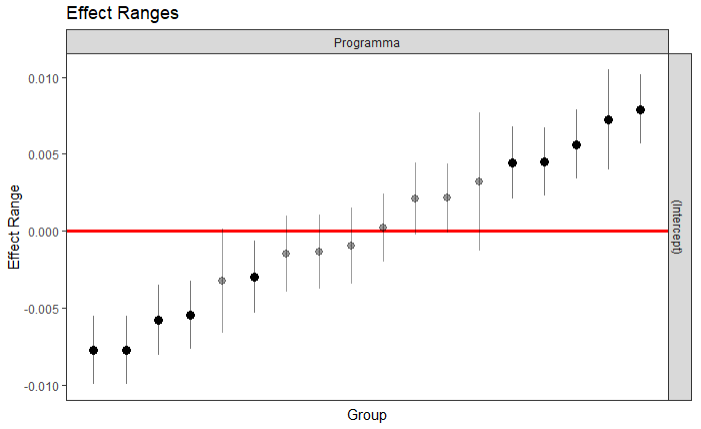
\includegraphics[width=0.7 \linewidth]{multi3.png}
    \label{fig:em}
    \caption{Grafico per la visualizzazione della significatività dell'effetto casuale di gruppo $a_j$.}
\end{figure}
\textbf{Modello 2}: Coefficiente $\sim$  Picco Press. (140) + Media Press.(2300) + Picco Press. (2300) + Temperatura + Picco Coppia Finale + (1$\mid$Programma)
{\begin{table}[h] 
\centering
\begin{tabular}[t]{lccc}
\toprule 
Variabile&$Pr(> |t|)$\\
\midrule 
\textbf{Intercetta}&$<$2e-16 ***&\\
\textbf{Picco Press. (140)}&$<$2.2e-16 ***\\ 
\textbf{Media Press. (2300)}&$<$2.2e-16 ***\\ 
\textbf{Picco Press. (2300)}&$<$2.2e-16 ***\\ 
\textbf{Temperatura}&0.6196549\\
\textbf{Picco Coppia Finale}&0.0001283 ***\\
\bottomrule 
\end{tabular}
\end{table}}\\
La variabile "Temperatura", in questo preciso caso, non è statisticamente significativa per la previsione. L'indice di bontà di adattamento ($R^2$) è sempre eccellente (0.939), e il coefficiente di correlazione intraclasse (ICC) è ancora moderato (0.797), confermando la presenza di una gerarchia meno sistematica nei dati riguardati la pressione. Anche qui, nonostante il minor livello di varianza intraclasse, possono essere individuati 10 cluster di produzione.
\begin{figure}[H]
    \centering
    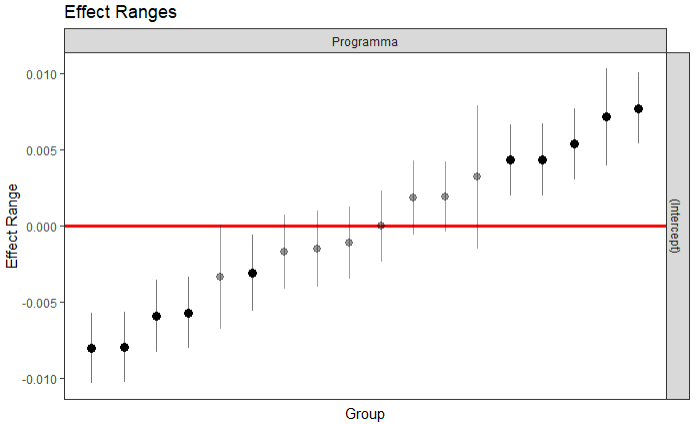
\includegraphics[width=0.7 \linewidth]{multi4.png}
    \label{fig:em}
    \caption{Grafico per la visualizzazione della significatività dell'effetto casuale di gruppo $a_j$.}
\end{figure}
\subsection{Conlclusioni sui modelli predittivi}
Tutti i modelli proposti sono in grado di prevedere il coefficiente di perdita con un'accuratezza accettabile: il minimo valore dell'indice di bontà di adattamento è 0.7058, ottenuto con una regolarizzazione di tipo \textit{Lasso}. Le regressioni regolarizzate risentono negativamente di un'eccessiva collinearità della matrice del disegno - come dimostrato empiricamente da Weisberg \cite{Wei}\cite{Wei1} -, e questo viene confermato dal fatto che anche l'$R^2$ prodotto al metodo \textit{Ridge} non sia eccellente: 0.845. Per questa ragione, le tecniche di \textit{shrinkage} sono sconsigliate.\\
Il modello migliore ($R^2=0.9508$) per la previsione di $\alpha$ consiste nella regressione lineare classica basato sulla combinazione di alcune variabili di pressione ("Picco Press. (140)", "Media Press.(2300)","Picco Press. (2300)"), temperatura e picco di coppia finale. Segue il modello OLS che include le stesse variabili di quello appena citato, ecceto per quanto riguarda il picco della coppia finale, sostituito dalla media della coppia finale. Pertanto, le regressioni lineari multiple basate sulle misurazioni di pressione in entrambe le fasi si rivelano essere le metodologie più accurate per la descrizione della variabile target. La seconda classe di metodi, in ordine di prestazione, è quella dei modelli multilivello, che, riuscendo a catturare gli effetti randomici propri dei diversi contesti di produzione, ottengono valori di $R^2$ compresi fra un minimo di 0.918 (quando la regressione è basata su grandezze di portata) e un massimo di 0.939 (in corrispondenza delle colonne di pressione). Nell'ambito di tali modelli misti, è interessante nota come quelli basati sulle misurazioni di pressione mostrino sempre un coefficiente ICC molto minore, quindi una struttura gerarchica meno evidente, ma un numero di cluster di produzione sempre maggiore.
In ogni caso, il grande problema di multicollinearità non ha permesso di utilizzare congiuntamente sia le variabili di portata e pressione che quelle relative alla coppia finale, né di condurre una \textit{feature selection} esplicita, obbligando una dispendiosa serie di tentativi di selezione manuale. 
%----------------------------------------------------------------------------------------
\section*{Codice}
L'intero codice, implementato con linguaggi \texttt{Python} e \texttt{R}, è disponibile al link: \url{https://github.com/RCrvro/Industry-Lab---Progetto}.
%----------------------------------------------------------------------------------------
%	REFERENCE LIST
%----------------------------------------------------------------------------------------
\newpage
\phantomsection
\bibliographystyle{unsrt}
\begin{thebibliography}{9}

\bibitem{El} 
T. Hastie, R. Tibshirani, J. Friedman; \textit{"The Elements of Statistical Learning: Data Mining, Inference, and Prediction"}, Stanford University, Stanford, 2009. 

\bibitem{Ridge}
A.E. Hoerl, R.W. Kennard; \textit{Ridge regression: Biased estimation for nonorthogonal problems}, in \textit{Technometrics}, vol. 42, n. 1, pp. 80–86, 1970.

\bibitem{Lasso}
R. Tibshirani; \textit{Regression Shrinkage and Selection via the lasso} in \textit{Journal of the Royal Statistical Society. Series B (methodological)}, 1996.

\bibitem{Multil}
S. W. Raudenbush, A. S. Bryk; \textit{Hierarchical linear models : applications and data analysis methods (2. ed., [3. Dr.] ed.)}, Thousand Oaks, CA [u.a.]: Sage Publications, 2002.

\bibitem{Multil1}
B. G. Tabachnick, L. S. Fidell; \textit{Using multivariate statistics (5th ed.)}, 2007.
 
\bibitem{Wei} 
\href{https://arxiv.org/pdf/math/0406473.pdf}{Discussione di Weisberg, su B. Efron, T. Hastie, I. Johnstone, R. Tibshirani; \textit{"Least Angle Regression"}, nella rivista \textit{"Annals of Statistics."}, 32 (2): pp. 407–499.} 

\bibitem{Wei1} 
S. Weisberg; \textit{Applied Linear Regression}, Wiley, New York, 1980.

\bibitem{PD} 
\href{https://plotly.com}{"Documentazione ufficiale di Plotly-Dash"}, 2020.

\bibitem{AK} 
\href{https://kafka.apache.org}{Apache Software Foundation, "Documentazione ufficiale di Apache Kafka"}, 2017.

\end{thebibliography}
%----------------------------------------------------------------------------------------

\end{document}
